\section{O-MCTS}
\label{sec:planning}

We propose O-MCTS, a novel algorithm that simulates the use of subgoals by
planning over options using MCTS, enabling the otherwise infeasible use of
options in complex MDPs\@. The resulting algorithm achieves higher scores than
MCTS on complex games that have several subgoals. It works as follows: like in
MCTS, a tree of states is built by simulating game plays. The algorithm chooses
options instead of actions. When an option is chosen, the actions returned by
its policy are used to build the tree. When an option is finished a new option
has to be chosen, which enables the tree to branch on that point. Since
traditional MCTS branches on each action, whereas O-MCTS only branches when an
option is finished, deeper search trees can be built in the same amount of time.
This section describes how the process works in more detail.

\begin{figure}
	\centering
	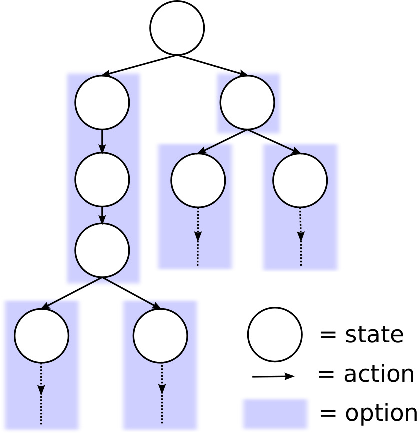
\includegraphics[width=.4\columnwidth]{includes/omcts-eps-converted-to.pdf}
	\caption{The search tree constructed by O-MCTS\@. In each blue box, one
	option is followed. The arrows represent actions chosen by the option. An
	arrow leading to a blue box is an action chosen by the option represented by
	that box.}
\label{fig:omcts-tree}
\end{figure}


The tree representation of an O-MCTS tree is the same as in MCTS\@: a node
represents a state, a connection represents an action. An option spans several
actions and therefore several nodes in the search tree, as shown in
Figure~\ref{fig:omcts-tree}. We introduce a change in the expansion and
selection strategies, which select options rather than actions. When a node has
an unfinished option, the next node will be created using an action selected by
that option. When a node contains a finished option (the current state satisfies
its termination condition $\beta$), a new option can be chosen by the expansion
or selection strategy. The search tree can only branch when an option is
finished.

\begin{algorithm}[h]
	\caption{$\mathsf{O-MCTS}(O, r, t, d)$}
\label{alg:omcts}
	\begin{algorithmic}[1]
		\State $C_{s \in S} \gets \emptyset$ \Comment{$\mathbf{c}_s$ is the set of children nodes of $s$}
		\State $\mathbf{o} \gets \emptyset$ \Comment{$o_s$ will hold the option followed in $s$}
		\While {$time\_taken < t$} \label{alg:omcts:mainloop}
			\State $s \gets r$ \Comment{start from root node}
			\While {$\neg \mathsf{stop}(s, d)$} \label{alg:omcts:innerloop}
				\If{$s \in \beta(o_s)$} \label{alg:omcts:sp} \Comment{if option stops in state $s$}
					\State $\mathbf{p}_s \gets \cup_o (s \in I_{o \in O})$ \Comment{$\mathbf{p}_s$ = available options}
				\Else
					\State $\mathbf{p}_s \gets \{o_s\}$ \Comment{continue with current option}
				\EndIf \label{alg:omcts:ep}
				\State $\mathbf{m} \gets \cup_o (o_{s \in \mathbf{c}_s})$ \Comment{set $\mathbf{m}$ to expanded options} \label{alg:omcts:m}
				\If{$\mathbf{p}_s = \mathbf{m}$} \Comment{if all options are expanded}
					\State $s' \gets \max_{c \in \mathbf{c}_s} \mathsf{uct}(s, c)$ \label{alg:omcts:uct} 
						\Comment{Eq.~\ref{eq:uct}}
					\State $s \gets s'$ \label{alg:omcts:ss} 
						\Comment{continue loop with child}
				\Else \label{alg:omcts:sexpand}
					\State $\omega \gets \mathsf{random\_element}(\mathbf{p}_s - \mathbf{m})$ 
					\State $a \gets \mathsf{get\_action}(\omega, s)$ 
					\State $s' \gets \mathsf{expand}(s, a)$ 
						\Comment{create child $s'$ using $a$}
						\State $\mathbf{c}_s \gets \mathbf{c}_s \cup \{s'\}$ \Comment{add to set of children}
					\State $o_{s'} \gets \omega$
					\State \textbf{break} \label{alg:omcts:break}
				\EndIf \label{alg:omcts:eexpand}
			\EndWhile
			\State $\delta \gets \mathsf{rollout}(s')$ \label{alg:omcts:rollout}
				\Comment{simulate until $\mathsf{stop}$}
			\State $\mathsf{back\_up}(s', \delta)$ \label{alg:omcts:backup}
				\Comment{save reward to parent nodes (Eq.~\ref{eq:backup})}
		\EndWhile
		\State \Return{$\mathsf{get\_action}(\max_{o \in \mathbf{c}_r} \mathsf{value}(o), r)$}
	\end{algorithmic}
\end{algorithm}
%\begin{figure}
%	\centering
%	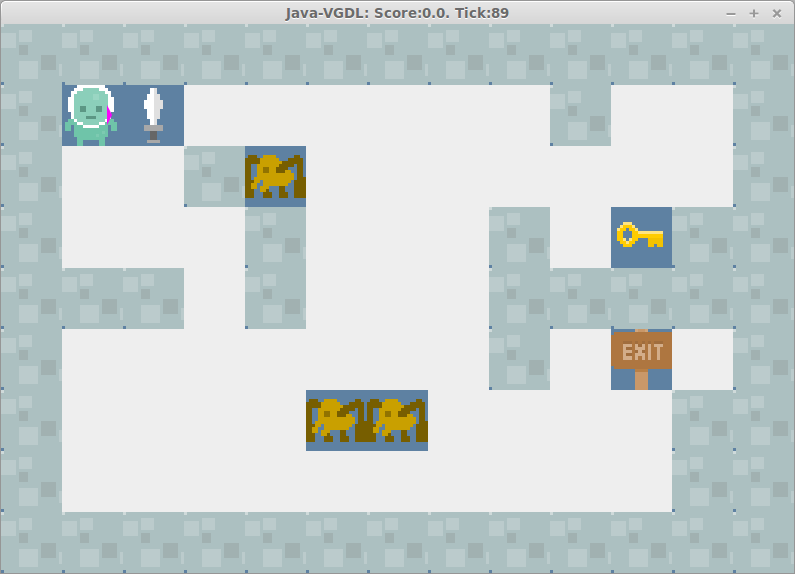
\includegraphics[width=\columnwidth]{includes/zelda}
%	\caption{Visual representation of the game \textit{zelda}.}
%\label{fig:zelda}
%\end{figure}

We describe O-MCTS in Algorithm~\ref{alg:omcts}. It is invoked with a set of
options $O$, a root node $r$, a maximum runtime $t$ in milliseconds and a
maximum search depth $d$. Two variables are instantiated. $C_s$ is a set of
sets, containing the set of child nodes for each node. The set $\mathbf{o}$
contains which option is followed for each node. The main loop starts at 
line~\ref{alg:omcts:mainloop}, which keeps the algorithm running until time runs out.
The inner loop runs until a node $s$ is reached that meets a stop criterion
defined by the function \textsf{stop}, or a node is expanded into a new node.
In lines~\ref{alg:omcts:sp} until~\ref{alg:omcts:ep}, $\mathbf{p}_s$ is set to
all options that are available in $s$. If an option has not finished,
$\mathbf{p}_s$ contains only the current option. Otherwise, it contains all the
options $o$ that have state $s$ in their initiation set $I_o$. For example, the
agent is playing \textit{zelda} and the current state $s$ shows no NPCs on
screen. If $o$ is the \textit{AvoidNearestNpcOption}, $I_o$ will not contain
state $s$, because there are no NPCs on screen, rendering $o$ useless in state
$s$. $\mathbf{p}_s$ will thus not contain option $o$.

O-MCTS consists of the same four phases as MCTS\@. In line~\ref{alg:omcts:m},
$\mathbf{m}$ is set to the set of options chosen in the children of state $s$.
If $\mathbf{p}_s$ is the same set as $\mathbf{m}$, i.e., all possible options
have been explored at least once in node $s$, a new node $s'$ is \emph{selected}
by \textsf{uct}. In line~\ref{alg:omcts:ss}, $s$ is instantiated with the new
node $s'$, continuing the inner loop using this node.  Else, some options are
apparently unexplored in node $s$. It is \emph{expanded} with a random,
currently unexplored option by lines~\ref{alg:omcts:sexpand}
to~\ref{alg:omcts:eexpand}. After expansion or when the stop criterion is met,
the inner loop is stopped and a \emph{rollout} is done, resulting in score
difference $\delta$. This score difference is \emph{backed up} to the parent
nodes of $s$ using the backup function, after which the tree traversal restarts
with the root node $r$.

A number of functions is used by Algorithm~\ref{alg:omcts}. The function
\textsf{stop} returns true when either the game ends in state $s$ or the maximum
depth is reached in $s$. The function \textsf{get\_action} lets option $\omega$
choose the best action for the state in node $s$, The function \textsf{expand}
creates a new child node $s'$ for node $s$. $s'$ contains the state that is
reached when action $a$ is applied to the state in node $s$. Typically, the
\textsf{rollout} function chooses random actions until \textsf{stop} returns
true, after which the difference in score achieved by the rollout is returned.
In O-MCTS however, \textsf{rollout} always applies actions chosen by option $o$
first and applies random actions after $o$ is finished. The \textsf{back\_up}
function traverses the tree through all parents of $s$, updating their expected
value. In contrast to traditional MCTS, which backs up the mean value of the
reward to all parent nodes, a discounted value is backed up. The backup function
for updating the value of ancestor node $s$ when a reward is reached in node $s'$
looks like this:
\begin{equation}
	\label{eq:backup}
	v_s \gets v_s + \delta\gamma^{d_{s'}-d_{s}},
\end{equation}
where $\delta$ is the reward that is being backed up, $v_s$ is the value of node
$s$. $d_s$ and $d_{s'}$ are the node depths of tree nodes $s$ and $s'$. Thus, a
node that is a further ancestor of node $s'$ will be updated with a smaller
value.

When the time limit is reached, the algorithm chooses an option from the
children of the root node, $\mathbf{c}_r$, corresponding to the child node with the
highest expected value. Subsequently, the algorithm returns the action that is
selected by this option for the state in the root node. This action is applied
to the game.

In the next state, the algorithm restarts by creating a new root node from
this state. Note that since O-MCTS always returns the action chosen by the best
option at that moment, the algorithm uses interruption.

We expect that since this implementation of MCTS with options reduces the
branching factor of the tree, as can be seen in figure~\ref{fig:omcts-tree}, the
algorithm can do a deeper tree search.  Furthermore, we expect that the
algorithm will be able to identify and meet a game's subgoals by using options.
In the experiments section we show results that support our expectations.
